\documentclass[a4paper,
fontsize=11pt,
%headings=small,
oneside,
numbers=noperiodatend,
parskip=half-,
bibliography=totoc,
final
]{scrartcl}

\usepackage{synttree}
\usepackage{graphicx}
\setkeys{Gin}{width=.6\textwidth} %default pics size

\graphicspath{{./plots/}}
\usepackage[english]{babel}
\usepackage[T1]{fontenc}
%\usepackage{amsmath}
\usepackage[utf8x]{inputenc}
\usepackage [hyphens]{url}
\usepackage{booktabs} 
\usepackage[left=2.4cm,right=2.4cm,top=2.3cm,bottom=2cm,includeheadfoot]{geometry}
\usepackage{eurosym}
\usepackage{multirow}
\usepackage[english]{varioref}
\setcapindent{1em}
\renewcommand{\labelitemi}{--}
\usepackage{paralist}
\usepackage{pdfpages}
\usepackage{lscape}
\usepackage{float}
\usepackage{acronym}
\usepackage{eurosym}
\usepackage[babel]{csquotes}
\usepackage{longtable,lscape}
\usepackage{mathpazo}
\usepackage[flushmargin,ragged]{footmisc} % left align footnote

\usepackage{listings}

\urlstyle{same}  % don't use monospace font for urls

\usepackage[fleqn]{amsmath}

%adjust fontsize for part

\usepackage{sectsty}
\partfont{\large}

%Das BibTeX-Zeichen mit \BibTeX setzen:
\def\symbol#1{\char #1\relax}
\def\bsl{{\tt\symbol{'134}}}
\def\BibTeX{{\rm B\kern-.05em{\sc i\kern-.025em b}\kern-.08em
    T\kern-.1667em\lower.7ex\hbox{E}\kern-.125emX}}

\usepackage{fancyhdr}
\fancyhf{}
\pagestyle{fancyplain}
\fancyhead[R]{\thepage}

%meta
%meta

\fancyhead[L]{Snowden Commons \\ %author
LIBREAS. Library Ideas, 26 (2014). % journal, issue, volume.
\href{http://nbn-resolving.de/urn:nbn:de:kobv:11-100222701
}{urn:nbn:de:kobv:11-100222701}} % urn
\fancyhead[R]{\thepage} %page number
\fancyfoot[L] {\textit{Creative Commons BY 3.0}} %licence
\fancyfoot[R] {\textit{ISSN: 1860-7950}}

\title{\LARGE{From the Snowden Files to the Snowden Commons: The Library as a Civic Hub}} %title %title
\author{Snowden Commons} %author

\setcounter{page}{65}

\usepackage[colorlinks, linkcolor=black,citecolor=black, urlcolor=blue,
breaklinks= true]{hyperref}

\date{}
\begin{document}

\maketitle
\thispagestyle{fancyplain} 

%abstracts

%body
\emph{Vorbemerkung von Ben Kaden}

Im Juli 2014 erschien im Online-Magazin \enquote{Berliner Gazette} ein
programmatischer Aufruf des Herausgebers Krystian Woznicki:
\enquote{Open the Snowden Files!} Anfang Dezember veröffentlichte die
Frankfurter Allgemeine Zeitung ein Interview mit Glenn Greenwald, in dem
dieser diese Öffnung ein Stück weit ankündigte:

\begin{quote}
FAZ: Snowdens Archiv wird öffentlich?

Greenwald: So ist es. Selbst wenn sich zehn Journalisten rund um die Uhr
damit beschäftigen, können sie immer noch Dinge übersehen, die andere
entdecken. Ich habe auch ein persönliches Motiv: Dieses Archiv lässt
mich nicht los. Wenn ich an etwas anderem arbeite, habe ich immer ein
schlechtes Gewissen und denke: Da gibt es noch etwas, von dem die Welt
wissen sollte. (Greenwald, Schaer)
\end{quote}

Nun wird der Konsultationsraum, den The Intercept in New York für eine
Auseinandersetzung mit dem Snowden-Material bereitzustellen plant, nicht
gerade eine Bibliothek sein. Ent\-sprech\-end bleibt trotz dieser Bemühungen
die Forderung Krystian Woznickis aktuell, der in seinem überaus intensiv
rezipierten Beitrag unter anderem folgende Überlegung ins Spiel brachte:

\begin{quote}
Drittens müsste sichergestellt werden, dass die Dateien in einer Art und
Weise zu\-gäng\-lich gemacht werden, die auch die Anonymität der User
schützt. Man will brisante Dateien nicht auf dem persönlichen Computer
haben, sondern in der Cloud, an einem öffentlich bekannten Ort, der
einen gesicherten Zugang erlaubt. Doch wer soll die Dateien dann hosten?
Ideal wäre eine öffentliche Institution, zum Beispiel eine Bibliothek.
(Woznicki)
\end{quote}

Dieses Ideal wirklich und produktiv zu adressieren war dann auch wenig
überraschend ein Arbeitsschwerpunkt des ‚Publics in Peril`-Tracks auf
der Slow-Politics-Konferenz in Berlin im November 2014. Über gut zwei
Tage erörterte eine kleine Gruppe von Akteuren mit unterschiedlichem
Hintergrund die Idee, wie sich überhaupt eine Relation zwischen dem
Snowden-Material und der Institution Bibliothek herstellen lässt. Neben
einer kurzen Präsentation erster Ergebnisse und einer Podiumsdiskussion
von Ben Kaden (LIBREAS) mit Geert Lovink (Institute of Network Cultures)
zum Thema am Abschlusstag der Konferenz (vgl. Krempl, 2014) entstand
eine Art Programmpapier, das wir an dieser Stelle gern dokumentieren.
Die abgebildete Fassung ist eine durchgesehene Version des Textes aus
der Ergebnisdokumentation zur SLOW POLITICS. Berliner Gazette Conference
2014.

\begin{figure}[htbp]
\centering
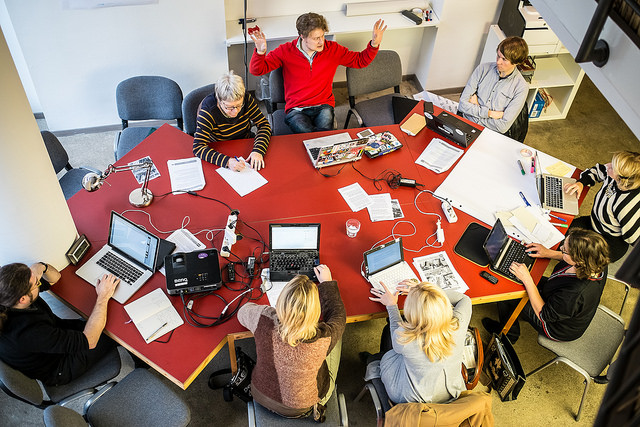
\includegraphics{flickr.jpg}
\caption{Arbeit am Snowden-Papier. Andi Weiland \textbar{}
berlinergazette.de (CC by),
\url{https://www.flickr.com/photos/berlinergazette/15759121896/}}
\end{figure}

Berliner Gazette: SLOW POLITICS. Berliner Gazette Conference 2014.
Results: Projects \& Documents.
\url{http://berlinergazette.de/wp-content/uploads/Snowden-Commons.pdf}

Greenwald, Glenn; Schaer, Ursula: Und dann traf ich den Mann mit dem
Zauberwürfel. In: Frankfurter Allgemeine Zeitung / faz.net, 03.12.2014
\url{http://www.faz.net/aktuell/feuilleton/glenn-greenwald-erzaehlt-ueber-seine-arbeit-mit-edward-snowden-13300668.html}

Krempl, Stefan: Ruf nach Veröffentlichung der Snowden-Papiere wird
lauter. In: heise.de, 16.11.2014,
\url{http://www.heise.de/newsticker/meldung/Ruf-nach-Veroeffentlichung-der-Snowden-Papiere-wird-lauter-2457781.html}

Woznicki, Krystian: Open the Snowden Files! Das öffentliche Interesse am
freien Zugang zu den Dokumenten der NSA-Gate. In: Berliner Gazette,
09.07.2014, \url{http://berlinergazette.de/open-the-snowden-files/}

\section*{From the Snowden Files to the Snowden Commons: The
Library as a Civic Hub}\label{from-the-snowden-files-to-the-snowden-commons-the-library-as-a-civic}

PART ONE: What's the problem?

\begin{itemize}
\item
  Citizen engagement in the \enquote{Post-Snowden} world
\item
  From the right to privacy to participatory autonomy
\item
  The library to the rescue
\item
  Security: Theirs and ours
\end{itemize}

PART TWO: What do we propose?

\section*{PART ONE: What's the
problem?}\label{part-one-whats-the-problem}

\subsection*{Citizen engagement in the \enquote{Post-Snowden}
World}\label{citizen-engagement-in-the-post-snowden-world}

The massive disclosure of secret NSA documents by Edward Snowden has
created an epochal opportunity for dialogue and debate, not only about
the nature of state surveillance and the right to privacy in the digital
age, but also about human rights and the future of democracy. We believe
that the Snowden files represent a crucial part of the World Heritage of
Contemporary Documentation: the essential texts citizens must have the
right to access so they can fully participate in a democratic society,
which is based on participatory and informed decision making. If this
is, indeed, a \enquote{Post-Snowden} era, then we all must have the
right to access the documents that initiated this new age.

Thus far, the Snowden files have inspired collaborations of experts,
policy-makers, journalists, activists, artists and concerned citizens.
We believe that these critical alliances demonstrate the potential of
the Snowden files to mobilize a broad public engagement. New models of
access and participation are needed. How can we support, build on and
expand the existing initiatives to include the wider variety of people
affected and concerned by these revelations and their implications, but
who, at present, are not active?

Most citizens have difficulty imagining the scope of the problem and how
it is affecting their lives and communities. It would be comfortable to
assume that the reason that the population at large has not shown wide
and sustained outrage after the Snowden revelations, has not engaged
with the released documents, and has not acted upon them, is simply
apathy, hopelessness and a sense of defeat and resignation. We insist
that the underacknowledged reason for this situation is that we have
inadequate public institutions for sharing this information in a way
that makes it genuinely accessible and understandable to everyone,
public institutions providing spaces for many forms of collaboration and
mobilization for collective action.

Today, just a few people actually access and engage with the Snowden
files, which are often confusing or inscrutable to non-specialists. For
this reason, we propose a renewed role for the public library as a place
to host not only the revealed files, but also organize, curate and care
for them so as to make control over and effective use of publicly
relevant information more tangible. In a democratic civic society,
access to the contemporary document heritage is enshrined in the mission
of libraries. Furthermore, the public library's democratic potential as
a safe and widely accessible space where people come together and
exchange ideas can help us transform this dauntingly huge pool of data
into tangible, public and actionable information. The public library
thus assumes an active role of a platform where problems and solutions
are recognized and articulated through the processes of citizen
participation. The question why the revelations matter for each of us
individually and for all of us collectively is then answered in a way
that can lead to sustainable and concrete collective action.

\subsection*{From the right to privacy to participatory
autonomy}\label{from-the-right-to-privacy-to-participatory-autonomy}

So far, citizens have been trapped between two strategies for defending
themselves from the forms of surveillance implied in the Snowden files,
both of which tend to be difficult for common citizens to participate in
because they require specialized technical or policy knowledge. On the
one hand, individuals have been encouraged to use new digital privacy
tools and techniques to create a wall between themselves and the
watchers (but is this a solution for everyone?).

On the other, some activists, organizations and human rights advocates
have sought to compel governments to better protect citizens' rights
through lobbying, legal action and constitutional challenges (but what
to do when the government is the watcher?). But there is a third option,
one that complements and supports the other two while creating something
new. We must re-create public spaces where citizens can learn about the
threat they face and come up with common, workable solutions: a place to
deliberate not only about how we are affected as individuals, but also
as a society and as communities, different communities being affected in
different ways, and what multiple perspectives different people and
different communities take on surveillance. In this way we can build a
solid and sustained public dialogue about security, surveillance,
privacy and autonomy.

We envision the public library as a space where social movements are
structured through sharing interests, information, strategies, tactics
and tools. We call upon librarians to facilitate the publics'
reclaimation of the information that impacts all of us.

Why? Because the \enquote{right to privacy} is not simply a personal
matter of the individual; it is a societal challenge which requires
society-level solutions. Further, human rights are not only something
granted under constitutional and international law; they must be
continuously demanded, negotiated, and constantly rebuilt from society's
grassroots. For instance, while article 5 of the German Constitution
guarantees the right of each person to \enquote{freely express and
disseminate their opinions in speech, writing, and pictures and to
inform themselves without hindrance from generally accessible sources},
such a right must be activated by citizens to be meaningful, effective
and transformative.

To confront the new powers of surveillance we need to think broadly
about building \enquote{zones of autonomy}: autonomy of the individual,
autonomy for communities, autonomy for society. The principle of
autonomy translates the ideal of privacy into concrete goals grounded in
human rights.

Privacy and autonomy are essential components of a functional and
vibrant democracy; without them critical citizenship is not possible. A
library could be an autonomous zone proper, librarians its caretakers.
We need to create and re-imagine public institutions to serve this
purpose in the digital age, to make information widely accessible, truly
common and operative.

\subsection*{The library to the rescue}\label{the-library-to-the-rescue}

Here is where the library comes in. In contrast to the variety of
websites that now house the publicly-accessible documents in the Snowden
files\footnote{vgl. die Sammlung bei cryptome.org:
  http://cryptome.org/2013/11/snowden-tally.htm}, and in contrast to
journalism, which has its own set of institutional, editorial and
financial pressures, the library provides:

\begin{itemize}
\item
  An open, free and accessible public institution for people to access
  and interpret the material, anonymously if they so choose
\item
  A trusted public institution with a long history and legacy of
  protecting and advancing the right to information
\item
  A physical space for multiple, diverse communities to access a common
  space, to learn from one another, and to develop and share rich,
  collaborative tools for accessing particular topics of interest
  (e.g.~indexing enables people to easily find information on a
  particular issue, visualizations allow for a better understanding of
  links)
\item
  A venue where experts, activists and advocates who have advanced data
  skills and specialist knowledge can interact with concerned members of
  the public
\item
  Institutional sustainability and long-term access to the documents
  into the future
\item
  Public ownership over data, which ensures citizens are legally
  protected and that information can serve the public interest
\item
  Qualified staff skilled in providing access to information, who can
  facilitate the contextualization and indexing of data, who can provide
  education, and who can support all different kinds of interaction with
  the material, for instance scholarly research
\item
  A venue for experimentation, collaboration, creativity, possibility
  and concerted collective action.
\end{itemize}

Where, other than the library, could migrants come together with
hackers, could poor people (who cannot afford computers or internet
access) come together with journalists, could researchers come together
with students? We envision the library as a unique and vital space where
multiple communities and individuals can work together on shared
concerns, with the support and facilitation of librarians and other
staff. In any case, such hopes will depend on robust public financial
support for public libraries, such that they can become the hubs of
citizenship, political engagement and autonomy in our troubled but
promising digital age.

\subsection*{Security: Theirs and ours}\label{security-theirs-and-ours}

The issue of safe, secure and legal access to sensitive information is
crucial. Both librarians and citizens should make full use of their
fundamental right of access to information without fear of legal
sanctions or surveillance. No one should be able to spy on them reading
the files, which is a risk with the use of online documents. Libraries
could provide for anonymous access to the Snowden files, with little or
no traces and strong data protection safeguards.

Furthermore, libraries would provide a precedent for handling the type
of information such as Snowden files and allow for testing the
participatory approaches to interacting with it and preserving it.
Thereby, a solid argument could be made for adopting a new model of
future leaks: not in the hands of one or a few, but in hands of the
public proper.

We see this as an important first step towards a culture of civic
autonomy and responsible open data. What would it take to turn the
library into an institution that could handle and make accessible a much
wider variety of leaked and sensitive data? What would it mean to see
the library as the hub for a democratic \enquote{civic intelligence}
movement that puts both \enquote{big data} and tools of mining and
engaging with it in the hands of the public? A public in power, not in
peril.

\section*{PART TWO: What do we propose?}\label{part-two-what-do-we-want-to-do}

How can we best integrate the Snowden Files into the library to achieve
the goals we have outlined here? Our answer may seem counter-intuitive
in this digital age of immaterial data and online communications: we
want to publish a book!

We intend to publish, in multiple volumes, the already-released Snowden
Files, and we are asking libraries to purchase a copy. We see this book
not only as an opportunity to maintain the documents for posterity; we
also want the physical books themselves to catalyze community dialogue,
debate and activism.

We understand ourselves both as creating a useful and important artifact
and archive, but also as making an important intervention in the
cultural and political climate of our times.

Why a physical book? There are a few reasons:

\begin{itemize}
\item
  It allows members of the public and researchers to safely, securely,
  privately and anonymously access the files in the library without fear
  of surveillance.
\item
  It will allow current and future researchers and users to cite and
  reference the Snowden Files with more certainty than online sources
  provide.
\item
  Many libraries are obligated to purchase new books, securing a wide
  distribution.
\item
  It will secure the files as a physical record for future generations.
\item
  Having multiple copies of the book distributed to thousands of
  libraries provides security against efforts by security services or
  others to destroy, tamper with or compromise the authenticity of the
  Snowden Files.
\item
  It will allow wider access to the files, which, while they can be
  found online, are currently scattered across multiple websites and
  sometimes difficult to access.
\item
  A comprehensive map of keywords and themes in the book to make the
  document navigable.
\item
  The book format will allow for additional contextual, editorial and
  expository information to be published alongside the Files, rendering
  them more accessible to non-specialists.
\item
  The Snowden Files are a crucial part of the World Heritage of
  Contemporary Documentation. As such, we see them as worthy of being
  honoured in a physical document.
\item
  Though we live in a digital culture, we also recognize that books have
  long been a key medium of social debate and an artifact around which
  people gather.
\item
  The book does not replace the online life of the Snowden Files, it
  augments and compliments it.
\end{itemize}

But we see the publication and distribution of the book as only the
first step. We have envisioned this book also as a catalyst or a
material that librarians and other stakeholders can use to bring people
together to debate, discuss and act on these key issues. As we move
forward with publication, we will also be developing and suggesting a
range of activities and uses.

These might include

\begin{itemize}
\item
  The publication of a regular (e.g.~quarterly, biannually)
  complimentary periodical which would provide analysis, updates and
  supplementary material to elucidate and animate various aspects of the
  Snowden Files,
\item
  A digital platform (or multiple digital platforms) to allow
  readers/users to share ideas, concerns, analysis, interpretations and
  disagreements --platforms that would allow users to communicate
  \enquote{in the margins} of the text and thereby connect their local
  issues to global problems,
\item
  Materials so that citizens can form reading groups or study circles,
  and also to connect those groups locally, nationally and
  internationally,
\item
  Invitations to create hackathons and public meetings to help index,
  interpret and respond to the leaks.
\end{itemize}

In short, we see the book and the library as a means to bring the
digital world down to the local level, to demystify and democratize
complex but important information, and to transform the Snowden Files
into the Snowden Commons. \enquote{Commons} are resources shared by
communities and which in turn help those communities sustain themselves;
think of a river which provides food and water for a village, but that
the village also cares for, cleans and watches over. The idea of the
Snowden Commons implies that the data contained in the files is a shared
resource through which we, as individuals and communities, gain agency
and empowerment in a democratic society. But, because they are a
commons, we must care for and maintain them, activate them and interpret
them.

We see this project as one step in this direction.

%autor

\end{document}
